% Created by tikzDevice version 0.10.1 on 2016-12-26 16:18:56
% !TEX encoding = UTF-8 Unicode
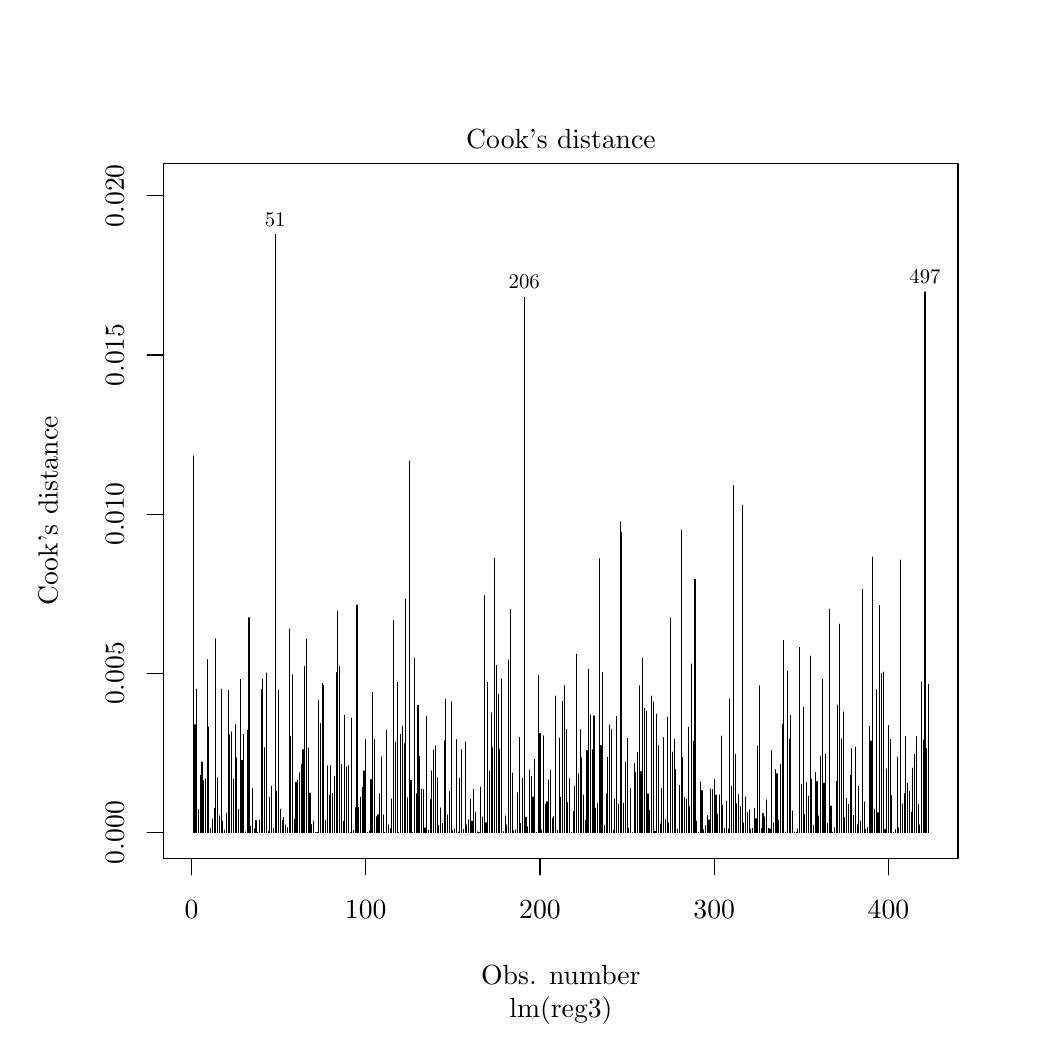
\begin{tikzpicture}[x=1pt,y=1pt]
\definecolor{fillColor}{RGB}{255,255,255}
\path[use as bounding box,fill=fillColor,fill opacity=0.00] (0,0) rectangle (361.35,361.35);
\begin{scope}
\path[clip] ( 49.20, 61.20) rectangle (336.15,312.15);
\definecolor{drawColor}{RGB}{0,0,0}

\path[draw=drawColor,line width= 0.4pt,line join=round,line cap=round] ( 59.83, 70.49) -- ( 59.83,206.61);

\path[draw=drawColor,line width= 0.4pt,line join=round,line cap=round] ( 60.46, 70.49) -- ( 60.46,109.48);

\path[draw=drawColor,line width= 0.4pt,line join=round,line cap=round] ( 61.09, 70.49) -- ( 61.09,122.34);

\path[draw=drawColor,line width= 0.4pt,line join=round,line cap=round] ( 61.72, 70.49) -- ( 61.72, 78.81);

\path[draw=drawColor,line width= 0.4pt,line join=round,line cap=round] ( 62.35, 70.49) -- ( 62.35, 91.12);

\path[draw=drawColor,line width= 0.4pt,line join=round,line cap=round] ( 62.98, 70.49) -- ( 62.98, 95.98);

\path[draw=drawColor,line width= 0.4pt,line join=round,line cap=round] ( 63.61, 70.49) -- ( 63.61, 89.21);

\path[draw=drawColor,line width= 0.4pt,line join=round,line cap=round] ( 64.24, 70.49) -- ( 64.24, 89.87);

\path[draw=drawColor,line width= 0.4pt,line join=round,line cap=round] ( 64.86, 70.49) -- ( 64.86,133.02);

\path[draw=drawColor,line width= 0.4pt,line join=round,line cap=round] ( 65.49, 70.49) -- ( 65.49,108.63);

\path[draw=drawColor,line width= 0.4pt,line join=round,line cap=round] ( 66.12, 70.49) -- ( 66.12, 72.10);

\path[draw=drawColor,line width= 0.4pt,line join=round,line cap=round] ( 66.75, 70.49) -- ( 66.75, 75.35);

\path[draw=drawColor,line width= 0.4pt,line join=round,line cap=round] ( 67.38, 70.49) -- ( 67.38, 79.31);

\path[draw=drawColor,line width= 0.4pt,line join=round,line cap=round] ( 68.01, 70.49) -- ( 68.01,140.47);

\path[draw=drawColor,line width= 0.4pt,line join=round,line cap=round] ( 68.64, 70.49) -- ( 68.64, 90.30);

\path[draw=drawColor,line width= 0.4pt,line join=round,line cap=round] ( 69.27, 70.49) -- ( 69.27, 76.52);

\path[draw=drawColor,line width= 0.4pt,line join=round,line cap=round] ( 69.90, 70.49) -- ( 69.90,122.35);

\path[draw=drawColor,line width= 0.4pt,line join=round,line cap=round] ( 70.53, 70.49) -- ( 70.53, 74.67);

\path[draw=drawColor,line width= 0.4pt,line join=round,line cap=round] ( 71.16, 70.49) -- ( 71.16, 71.34);

\path[draw=drawColor,line width= 0.4pt,line join=round,line cap=round] ( 71.79, 70.49) -- ( 71.79, 77.51);

\path[draw=drawColor,line width= 0.4pt,line join=round,line cap=round] ( 72.42, 70.49) -- ( 72.42,121.82);

\path[draw=drawColor,line width= 0.4pt,line join=round,line cap=round] ( 73.05, 70.49) -- ( 73.05,105.83);

\path[draw=drawColor,line width= 0.4pt,line join=round,line cap=round] ( 73.68, 70.49) -- ( 73.68,106.85);

\path[draw=drawColor,line width= 0.4pt,line join=round,line cap=round] ( 74.31, 70.49) -- ( 74.31, 89.80);

\path[draw=drawColor,line width= 0.4pt,line join=round,line cap=round] ( 74.94, 70.49) -- ( 74.94,109.54);

\path[draw=drawColor,line width= 0.4pt,line join=round,line cap=round] ( 75.57, 70.49) -- ( 75.57, 97.53);

\path[draw=drawColor,line width= 0.4pt,line join=round,line cap=round] ( 76.20, 70.49) -- ( 76.20, 78.90);

\path[draw=drawColor,line width= 0.4pt,line join=round,line cap=round] ( 76.83, 70.49) -- ( 76.83,125.86);

\path[draw=drawColor,line width= 0.4pt,line join=round,line cap=round] ( 77.46, 70.49) -- ( 77.46, 96.63);

\path[draw=drawColor,line width= 0.4pt,line join=round,line cap=round] ( 78.09, 70.49) -- ( 78.09,105.88);

\path[draw=drawColor,line width= 0.4pt,line join=round,line cap=round] ( 78.72, 70.49) -- ( 78.72, 70.76);

\path[draw=drawColor,line width= 0.4pt,line join=round,line cap=round] ( 79.35, 70.49) -- ( 79.35,107.46);

\path[draw=drawColor,line width= 0.4pt,line join=round,line cap=round] ( 79.98, 70.49) -- ( 79.98,148.13);

\path[draw=drawColor,line width= 0.4pt,line join=round,line cap=round] ( 80.60, 70.49) -- ( 80.60, 72.79);

\path[draw=drawColor,line width= 0.4pt,line join=round,line cap=round] ( 81.23, 70.49) -- ( 81.23, 86.50);

\path[draw=drawColor,line width= 0.4pt,line join=round,line cap=round] ( 81.86, 70.49) -- ( 81.86, 71.84);

\path[draw=drawColor,line width= 0.4pt,line join=round,line cap=round] ( 82.49, 70.49) -- ( 82.49, 74.87);

\path[draw=drawColor,line width= 0.4pt,line join=round,line cap=round] ( 83.12, 70.49) -- ( 83.12, 70.61);

\path[draw=drawColor,line width= 0.4pt,line join=round,line cap=round] ( 83.75, 70.49) -- ( 83.75, 75.10);

\path[draw=drawColor,line width= 0.4pt,line join=round,line cap=round] ( 84.38, 70.49) -- ( 84.38,122.13);

\path[draw=drawColor,line width= 0.4pt,line join=round,line cap=round] ( 85.01, 70.49) -- ( 85.01,125.96);

\path[draw=drawColor,line width= 0.4pt,line join=round,line cap=round] ( 85.64, 70.49) -- ( 85.64,101.22);

\path[draw=drawColor,line width= 0.4pt,line join=round,line cap=round] ( 86.27, 70.49) -- ( 86.27,128.14);

\path[draw=drawColor,line width= 0.4pt,line join=round,line cap=round] ( 86.90, 70.49) -- ( 86.90, 70.86);

\path[draw=drawColor,line width= 0.4pt,line join=round,line cap=round] ( 87.53, 70.49) -- ( 87.53, 83.31);

\path[draw=drawColor,line width= 0.4pt,line join=round,line cap=round] ( 88.16, 70.49) -- ( 88.16, 87.29);

\path[draw=drawColor,line width= 0.4pt,line join=round,line cap=round] ( 88.79, 70.49) -- ( 88.79, 71.98);

\path[draw=drawColor,line width= 0.4pt,line join=round,line cap=round] ( 89.42, 70.49) -- ( 89.42,286.64);

\path[draw=drawColor,line width= 0.4pt,line join=round,line cap=round] ( 90.05, 70.49) -- ( 90.05, 85.39);

\path[draw=drawColor,line width= 0.4pt,line join=round,line cap=round] ( 90.68, 70.49) -- ( 90.68,121.91);

\path[draw=drawColor,line width= 0.4pt,line join=round,line cap=round] ( 91.31, 70.49) -- ( 91.31, 78.95);

\path[draw=drawColor,line width= 0.4pt,line join=round,line cap=round] ( 91.94, 70.49) -- ( 91.94, 74.88);

\path[draw=drawColor,line width= 0.4pt,line join=round,line cap=round] ( 92.57, 70.49) -- ( 92.57, 75.97);

\path[draw=drawColor,line width= 0.4pt,line join=round,line cap=round] ( 93.20, 70.49) -- ( 93.20, 73.26);

\path[draw=drawColor,line width= 0.4pt,line join=round,line cap=round] ( 93.83, 70.49) -- ( 93.83, 72.25);

\path[draw=drawColor,line width= 0.4pt,line join=round,line cap=round] ( 94.46, 70.49) -- ( 94.46,144.11);

\path[draw=drawColor,line width= 0.4pt,line join=round,line cap=round] ( 95.09, 70.49) -- ( 95.09,105.25);

\path[draw=drawColor,line width= 0.4pt,line join=round,line cap=round] ( 95.72, 70.49) -- ( 95.72,127.51);

\path[draw=drawColor,line width= 0.4pt,line join=round,line cap=round] ( 96.35, 70.49) -- ( 96.35, 75.30);

\path[draw=drawColor,line width= 0.4pt,line join=round,line cap=round] ( 96.97, 70.49) -- ( 96.97, 88.61);

\path[draw=drawColor,line width= 0.4pt,line join=round,line cap=round] ( 97.60, 70.49) -- ( 97.60, 89.46);

\path[draw=drawColor,line width= 0.4pt,line join=round,line cap=round] ( 98.23, 70.49) -- ( 98.23, 92.02);

\path[draw=drawColor,line width= 0.4pt,line join=round,line cap=round] ( 98.86, 70.49) -- ( 98.86, 95.04);

\path[draw=drawColor,line width= 0.4pt,line join=round,line cap=round] ( 99.49, 70.49) -- ( 99.49,100.42);

\path[draw=drawColor,line width= 0.4pt,line join=round,line cap=round] (100.12, 70.49) -- (100.12,130.50);

\path[draw=drawColor,line width= 0.4pt,line join=round,line cap=round] (100.75, 70.49) -- (100.75,140.43);

\path[draw=drawColor,line width= 0.4pt,line join=round,line cap=round] (101.38, 70.49) -- (101.38,101.12);

\path[draw=drawColor,line width= 0.4pt,line join=round,line cap=round] (102.01, 70.49) -- (102.01, 84.78);

\path[draw=drawColor,line width= 0.4pt,line join=round,line cap=round] (102.64, 70.49) -- (102.64, 73.34);

\path[draw=drawColor,line width= 0.4pt,line join=round,line cap=round] (103.27, 70.49) -- (103.27, 74.60);

\path[draw=drawColor,line width= 0.4pt,line join=round,line cap=round] (103.90, 70.49) -- (103.90, 70.51);

\path[draw=drawColor,line width= 0.4pt,line join=round,line cap=round] (104.53, 70.49) -- (104.53, 70.52);

\path[draw=drawColor,line width= 0.4pt,line join=round,line cap=round] (105.16, 70.49) -- (105.16,118.30);

\path[draw=drawColor,line width= 0.4pt,line join=round,line cap=round] (105.79, 70.49) -- (105.79,109.90);

\path[draw=drawColor,line width= 0.4pt,line join=round,line cap=round] (106.42, 70.49) -- (106.42,124.42);

\path[draw=drawColor,line width= 0.4pt,line join=round,line cap=round] (107.05, 70.49) -- (107.05,123.68);

\path[draw=drawColor,line width= 0.4pt,line join=round,line cap=round] (107.68, 70.49) -- (107.68, 74.98);

\path[draw=drawColor,line width= 0.4pt,line join=round,line cap=round] (108.31, 70.49) -- (108.31, 94.57);

\path[draw=drawColor,line width= 0.4pt,line join=round,line cap=round] (108.94, 70.49) -- (108.94, 84.02);

\path[draw=drawColor,line width= 0.4pt,line join=round,line cap=round] (109.57, 70.49) -- (109.57, 94.63);

\path[draw=drawColor,line width= 0.4pt,line join=round,line cap=round] (110.20, 70.49) -- (110.20, 84.61);

\path[draw=drawColor,line width= 0.4pt,line join=round,line cap=round] (110.83, 70.49) -- (110.83, 90.74);

\path[draw=drawColor,line width= 0.4pt,line join=round,line cap=round] (111.46, 70.49) -- (111.46,128.25);

\path[draw=drawColor,line width= 0.4pt,line join=round,line cap=round] (112.09, 70.49) -- (112.09,150.48);

\path[draw=drawColor,line width= 0.4pt,line join=round,line cap=round] (112.71, 70.49) -- (112.71,130.46);

\path[draw=drawColor,line width= 0.4pt,line join=round,line cap=round] (113.34, 70.49) -- (113.34, 95.06);

\path[draw=drawColor,line width= 0.4pt,line join=round,line cap=round] (113.97, 70.49) -- (113.97, 74.57);

\path[draw=drawColor,line width= 0.4pt,line join=round,line cap=round] (114.60, 70.49) -- (114.60,112.89);

\path[draw=drawColor,line width= 0.4pt,line join=round,line cap=round] (115.23, 70.49) -- (115.23, 94.26);

\path[draw=drawColor,line width= 0.4pt,line join=round,line cap=round] (115.86, 70.49) -- (115.86, 94.70);

\path[draw=drawColor,line width= 0.4pt,line join=round,line cap=round] (116.49, 70.49) -- (116.49, 70.51);

\path[draw=drawColor,line width= 0.4pt,line join=round,line cap=round] (117.12, 70.49) -- (117.12,111.83);

\path[draw=drawColor,line width= 0.4pt,line join=round,line cap=round] (117.75, 70.49) -- (117.75, 71.31);

\path[draw=drawColor,line width= 0.4pt,line join=round,line cap=round] (118.38, 70.49) -- (118.38, 79.46);

\path[draw=drawColor,line width= 0.4pt,line join=round,line cap=round] (119.01, 70.49) -- (119.01,152.75);

\path[draw=drawColor,line width= 0.4pt,line join=round,line cap=round] (119.64, 70.49) -- (119.64, 79.57);

\path[draw=drawColor,line width= 0.4pt,line join=round,line cap=round] (120.27, 70.49) -- (120.27, 83.17);

\path[draw=drawColor,line width= 0.4pt,line join=round,line cap=round] (120.90, 70.49) -- (120.90, 86.78);

\path[draw=drawColor,line width= 0.4pt,line join=round,line cap=round] (121.53, 70.49) -- (121.53, 92.75);

\path[draw=drawColor,line width= 0.4pt,line join=round,line cap=round] (122.16, 70.49) -- (122.16,104.06);

\path[draw=drawColor,line width= 0.4pt,line join=round,line cap=round] (122.79, 70.49) -- (122.79, 70.51);

\path[draw=drawColor,line width= 0.4pt,line join=round,line cap=round] (123.42, 70.49) -- (123.42, 71.06);

\path[draw=drawColor,line width= 0.4pt,line join=round,line cap=round] (124.05, 70.49) -- (124.05, 89.64);

\path[draw=drawColor,line width= 0.4pt,line join=round,line cap=round] (124.68, 70.49) -- (124.68,121.16);

\path[draw=drawColor,line width= 0.4pt,line join=round,line cap=round] (125.31, 70.49) -- (125.31,104.09);

\path[draw=drawColor,line width= 0.4pt,line join=round,line cap=round] (125.94, 70.49) -- (125.94, 76.20);

\path[draw=drawColor,line width= 0.4pt,line join=round,line cap=round] (126.57, 70.49) -- (126.57, 76.94);

\path[draw=drawColor,line width= 0.4pt,line join=round,line cap=round] (127.20, 70.49) -- (127.20, 84.52);

\path[draw=drawColor,line width= 0.4pt,line join=round,line cap=round] (127.83, 70.49) -- (127.83, 97.80);

\path[draw=drawColor,line width= 0.4pt,line join=round,line cap=round] (128.46, 70.49) -- (128.46, 76.89);

\path[draw=drawColor,line width= 0.4pt,line join=round,line cap=round] (129.08, 70.49) -- (129.08, 70.53);

\path[draw=drawColor,line width= 0.4pt,line join=round,line cap=round] (129.71, 70.49) -- (129.71,107.49);

\path[draw=drawColor,line width= 0.4pt,line join=round,line cap=round] (130.34, 70.49) -- (130.34, 73.26);

\path[draw=drawColor,line width= 0.4pt,line join=round,line cap=round] (130.97, 70.49) -- (130.97, 71.82);

\path[draw=drawColor,line width= 0.4pt,line join=round,line cap=round] (131.60, 70.49) -- (131.60, 82.64);

\path[draw=drawColor,line width= 0.4pt,line join=round,line cap=round] (132.23, 70.49) -- (132.23,147.15);

\path[draw=drawColor,line width= 0.4pt,line join=round,line cap=round] (132.86, 70.49) -- (132.86,103.18);

\path[draw=drawColor,line width= 0.4pt,line join=round,line cap=round] (133.49, 70.49) -- (133.49,124.78);

\path[draw=drawColor,line width= 0.4pt,line join=round,line cap=round] (134.12, 70.49) -- (134.12, 70.51);

\path[draw=drawColor,line width= 0.4pt,line join=round,line cap=round] (134.75, 70.49) -- (134.75,105.99);

\path[draw=drawColor,line width= 0.4pt,line join=round,line cap=round] (135.38, 70.49) -- (135.38,108.91);

\path[draw=drawColor,line width= 0.4pt,line join=round,line cap=round] (136.01, 70.49) -- (136.01,102.61);

\path[draw=drawColor,line width= 0.4pt,line join=round,line cap=round] (136.64, 70.49) -- (136.64,154.87);

\path[draw=drawColor,line width= 0.4pt,line join=round,line cap=round] (137.27, 70.49) -- (137.27, 83.00);

\path[draw=drawColor,line width= 0.4pt,line join=round,line cap=round] (137.90, 70.49) -- (137.90,204.83);

\path[draw=drawColor,line width= 0.4pt,line join=round,line cap=round] (138.53, 70.49) -- (138.53, 89.40);

\path[draw=drawColor,line width= 0.4pt,line join=round,line cap=round] (139.16, 70.49) -- (139.16, 70.50);

\path[draw=drawColor,line width= 0.4pt,line join=round,line cap=round] (139.79, 70.49) -- (139.79,133.39);

\path[draw=drawColor,line width= 0.4pt,line join=round,line cap=round] (140.42, 70.49) -- (140.42, 84.51);

\path[draw=drawColor,line width= 0.4pt,line join=round,line cap=round] (141.05, 70.49) -- (141.05,116.50);

\path[draw=drawColor,line width= 0.4pt,line join=round,line cap=round] (141.68, 70.49) -- (141.68, 98.00);

\path[draw=drawColor,line width= 0.4pt,line join=round,line cap=round] (142.31, 70.49) -- (142.31, 86.21);

\path[draw=drawColor,line width= 0.4pt,line join=round,line cap=round] (142.94, 70.49) -- (142.94, 86.05);

\path[draw=drawColor,line width= 0.4pt,line join=round,line cap=round] (143.57, 70.49) -- (143.57, 72.14);

\path[draw=drawColor,line width= 0.4pt,line join=round,line cap=round] (144.20, 70.49) -- (144.20,112.48);

\path[draw=drawColor,line width= 0.4pt,line join=round,line cap=round] (144.82, 70.49) -- (144.82, 71.16);

\path[draw=drawColor,line width= 0.4pt,line join=round,line cap=round] (145.45, 70.49) -- (145.45, 82.35);

\path[draw=drawColor,line width= 0.4pt,line join=round,line cap=round] (146.08, 70.49) -- (146.08, 92.81);

\path[draw=drawColor,line width= 0.4pt,line join=round,line cap=round] (146.71, 70.49) -- (146.71,100.34);

\path[draw=drawColor,line width= 0.4pt,line join=round,line cap=round] (147.34, 70.49) -- (147.34,101.82);

\path[draw=drawColor,line width= 0.4pt,line join=round,line cap=round] (147.97, 70.49) -- (147.97, 90.24);

\path[draw=drawColor,line width= 0.4pt,line join=round,line cap=round] (148.60, 70.49) -- (148.60, 73.09);

\path[draw=drawColor,line width= 0.4pt,line join=round,line cap=round] (149.23, 70.49) -- (149.23, 79.38);

\path[draw=drawColor,line width= 0.4pt,line join=round,line cap=round] (149.86, 70.49) -- (149.86, 73.80);

\path[draw=drawColor,line width= 0.4pt,line join=round,line cap=round] (150.49, 70.49) -- (150.49,103.63);

\path[draw=drawColor,line width= 0.4pt,line join=round,line cap=round] (151.12, 70.49) -- (151.12,118.64);

\path[draw=drawColor,line width= 0.4pt,line join=round,line cap=round] (151.75, 70.49) -- (151.75, 76.80);

\path[draw=drawColor,line width= 0.4pt,line join=round,line cap=round] (152.38, 70.49) -- (152.38, 85.30);

\path[draw=drawColor,line width= 0.4pt,line join=round,line cap=round] (153.01, 70.49) -- (153.01,117.69);

\path[draw=drawColor,line width= 0.4pt,line join=round,line cap=round] (153.64, 70.49) -- (153.64, 71.24);

\path[draw=drawColor,line width= 0.4pt,line join=round,line cap=round] (154.27, 70.49) -- (154.27, 71.85);

\path[draw=drawColor,line width= 0.4pt,line join=round,line cap=round] (154.90, 70.49) -- (154.90,104.05);

\path[draw=drawColor,line width= 0.4pt,line join=round,line cap=round] (155.53, 70.49) -- (155.53, 70.62);

\path[draw=drawColor,line width= 0.4pt,line join=round,line cap=round] (156.16, 70.49) -- (156.16, 90.16);

\path[draw=drawColor,line width= 0.4pt,line join=round,line cap=round] (156.79, 70.49) -- (156.79,100.34);

\path[draw=drawColor,line width= 0.4pt,line join=round,line cap=round] (157.42, 70.49) -- (157.42, 71.68);

\path[draw=drawColor,line width= 0.4pt,line join=round,line cap=round] (158.05, 70.49) -- (158.05,103.24);

\path[draw=drawColor,line width= 0.4pt,line join=round,line cap=round] (158.68, 70.49) -- (158.68, 73.29);

\path[draw=drawColor,line width= 0.4pt,line join=round,line cap=round] (159.31, 70.49) -- (159.31, 75.06);

\path[draw=drawColor,line width= 0.4pt,line join=round,line cap=round] (159.94, 70.49) -- (159.94, 82.51);

\path[draw=drawColor,line width= 0.4pt,line join=round,line cap=round] (160.57, 70.49) -- (160.57, 74.58);

\path[draw=drawColor,line width= 0.4pt,line join=round,line cap=round] (161.19, 70.49) -- (161.19, 86.13);

\path[draw=drawColor,line width= 0.4pt,line join=round,line cap=round] (161.82, 70.49) -- (161.82, 77.84);

\path[draw=drawColor,line width= 0.4pt,line join=round,line cap=round] (162.45, 70.49) -- (162.45, 70.71);

\path[draw=drawColor,line width= 0.4pt,line join=round,line cap=round] (163.08, 70.49) -- (163.08, 70.54);

\path[draw=drawColor,line width= 0.4pt,line join=round,line cap=round] (163.71, 70.49) -- (163.71, 86.92);

\path[draw=drawColor,line width= 0.4pt,line join=round,line cap=round] (164.34, 70.49) -- (164.34, 76.14);

\path[draw=drawColor,line width= 0.4pt,line join=round,line cap=round] (164.97, 70.49) -- (164.97,156.08);

\path[draw=drawColor,line width= 0.4pt,line join=round,line cap=round] (165.60, 70.49) -- (165.60, 74.07);

\path[draw=drawColor,line width= 0.4pt,line join=round,line cap=round] (166.23, 70.49) -- (166.23,124.78);

\path[draw=drawColor,line width= 0.4pt,line join=round,line cap=round] (166.86, 70.49) -- (166.86, 92.66);

\path[draw=drawColor,line width= 0.4pt,line join=round,line cap=round] (167.49, 70.49) -- (167.49,113.77);

\path[draw=drawColor,line width= 0.4pt,line join=round,line cap=round] (168.12, 70.49) -- (168.12,101.21);

\path[draw=drawColor,line width= 0.4pt,line join=round,line cap=round] (168.75, 70.49) -- (168.75,169.62);

\path[draw=drawColor,line width= 0.4pt,line join=round,line cap=round] (169.38, 70.49) -- (169.38,130.88);

\path[draw=drawColor,line width= 0.4pt,line join=round,line cap=round] (170.01, 70.49) -- (170.01,120.55);

\path[draw=drawColor,line width= 0.4pt,line join=round,line cap=round] (170.64, 70.49) -- (170.64,100.61);

\path[draw=drawColor,line width= 0.4pt,line join=round,line cap=round] (171.27, 70.49) -- (171.27,125.98);

\path[draw=drawColor,line width= 0.4pt,line join=round,line cap=round] (171.90, 70.49) -- (171.90, 70.81);

\path[draw=drawColor,line width= 0.4pt,line join=round,line cap=round] (172.53, 70.49) -- (172.53, 76.49);

\path[draw=drawColor,line width= 0.4pt,line join=round,line cap=round] (173.16, 70.49) -- (173.16, 73.25);

\path[draw=drawColor,line width= 0.4pt,line join=round,line cap=round] (173.79, 70.49) -- (173.79,132.85);

\path[draw=drawColor,line width= 0.4pt,line join=round,line cap=round] (174.42, 70.49) -- (174.42,151.07);

\path[draw=drawColor,line width= 0.4pt,line join=round,line cap=round] (175.05, 70.49) -- (175.05, 92.01);

\path[draw=drawColor,line width= 0.4pt,line join=round,line cap=round] (175.68, 70.49) -- (175.68, 71.14);

\path[draw=drawColor,line width= 0.4pt,line join=round,line cap=round] (176.31, 70.49) -- (176.31, 71.50);

\path[draw=drawColor,line width= 0.4pt,line join=round,line cap=round] (176.93, 70.49) -- (176.93, 84.81);

\path[draw=drawColor,line width= 0.4pt,line join=round,line cap=round] (177.56, 70.49) -- (177.56,104.86);

\path[draw=drawColor,line width= 0.4pt,line join=round,line cap=round] (178.19, 70.49) -- (178.19, 73.77);

\path[draw=drawColor,line width= 0.4pt,line join=round,line cap=round] (178.82, 70.49) -- (178.82, 90.11);

\path[draw=drawColor,line width= 0.4pt,line join=round,line cap=round] (179.45, 70.49) -- (179.45,263.97);

\path[draw=drawColor,line width= 0.4pt,line join=round,line cap=round] (180.08, 70.49) -- (180.08, 76.03);

\path[draw=drawColor,line width= 0.4pt,line join=round,line cap=round] (180.71, 70.49) -- (180.71, 72.59);

\path[draw=drawColor,line width= 0.4pt,line join=round,line cap=round] (181.34, 70.49) -- (181.34, 93.06);

\path[draw=drawColor,line width= 0.4pt,line join=round,line cap=round] (181.97, 70.49) -- (181.97, 90.83);

\path[draw=drawColor,line width= 0.4pt,line join=round,line cap=round] (182.60, 70.49) -- (182.60, 83.36);

\path[draw=drawColor,line width= 0.4pt,line join=round,line cap=round] (183.23, 70.49) -- (183.23, 96.89);

\path[draw=drawColor,line width= 0.4pt,line join=round,line cap=round] (183.86, 70.49) -- (183.86, 70.54);

\path[draw=drawColor,line width= 0.4pt,line join=round,line cap=round] (184.49, 70.49) -- (184.49,127.15);

\path[draw=drawColor,line width= 0.4pt,line join=round,line cap=round] (185.12, 70.49) -- (185.12,106.29);

\path[draw=drawColor,line width= 0.4pt,line join=round,line cap=round] (185.75, 70.49) -- (185.75, 71.41);

\path[draw=drawColor,line width= 0.4pt,line join=round,line cap=round] (186.38, 70.49) -- (186.38,105.43);

\path[draw=drawColor,line width= 0.4pt,line join=round,line cap=round] (187.01, 70.49) -- (187.01, 80.80);

\path[draw=drawColor,line width= 0.4pt,line join=round,line cap=round] (187.64, 70.49) -- (187.64, 81.59);

\path[draw=drawColor,line width= 0.4pt,line join=round,line cap=round] (188.27, 70.49) -- (188.27, 89.50);

\path[draw=drawColor,line width= 0.4pt,line join=round,line cap=round] (188.90, 70.49) -- (188.90, 92.94);

\path[draw=drawColor,line width= 0.4pt,line join=round,line cap=round] (189.53, 70.49) -- (189.53, 75.60);

\path[draw=drawColor,line width= 0.4pt,line join=round,line cap=round] (190.16, 70.49) -- (190.16, 76.25);

\path[draw=drawColor,line width= 0.4pt,line join=round,line cap=round] (190.79, 70.49) -- (190.79,119.79);

\path[draw=drawColor,line width= 0.4pt,line join=round,line cap=round] (191.42, 70.49) -- (191.42, 71.30);

\path[draw=drawColor,line width= 0.4pt,line join=round,line cap=round] (192.05, 70.49) -- (192.05,104.64);

\path[draw=drawColor,line width= 0.4pt,line join=round,line cap=round] (192.68, 70.49) -- (192.68, 83.22);

\path[draw=drawColor,line width= 0.4pt,line join=round,line cap=round] (193.30, 70.49) -- (193.30,117.89);

\path[draw=drawColor,line width= 0.4pt,line join=round,line cap=round] (193.93, 70.49) -- (193.93,123.60);

\path[draw=drawColor,line width= 0.4pt,line join=round,line cap=round] (194.56, 70.49) -- (194.56,107.77);

\path[draw=drawColor,line width= 0.4pt,line join=round,line cap=round] (195.19, 70.49) -- (195.19, 81.30);

\path[draw=drawColor,line width= 0.4pt,line join=round,line cap=round] (195.82, 70.49) -- (195.82, 89.99);

\path[draw=drawColor,line width= 0.4pt,line join=round,line cap=round] (196.45, 70.49) -- (196.45, 70.52);

\path[draw=drawColor,line width= 0.4pt,line join=round,line cap=round] (197.08, 70.49) -- (197.08, 78.08);

\path[draw=drawColor,line width= 0.4pt,line join=round,line cap=round] (197.71, 70.49) -- (197.71, 87.30);

\path[draw=drawColor,line width= 0.4pt,line join=round,line cap=round] (198.34, 70.49) -- (198.34,134.99);

\path[draw=drawColor,line width= 0.4pt,line join=round,line cap=round] (198.97, 70.49) -- (198.97, 91.76);

\path[draw=drawColor,line width= 0.4pt,line join=round,line cap=round] (199.60, 70.49) -- (199.60,107.67);

\path[draw=drawColor,line width= 0.4pt,line join=round,line cap=round] (200.23, 70.49) -- (200.23, 97.56);

\path[draw=drawColor,line width= 0.4pt,line join=round,line cap=round] (200.86, 70.49) -- (200.86, 83.98);

\path[draw=drawColor,line width= 0.4pt,line join=round,line cap=round] (201.49, 70.49) -- (201.49, 74.99);

\path[draw=drawColor,line width= 0.4pt,line join=round,line cap=round] (202.12, 70.49) -- (202.12,100.16);

\path[draw=drawColor,line width= 0.4pt,line join=round,line cap=round] (202.75, 70.49) -- (202.75,129.53);

\path[draw=drawColor,line width= 0.4pt,line join=round,line cap=round] (203.38, 70.49) -- (203.38,112.99);

\path[draw=drawColor,line width= 0.4pt,line join=round,line cap=round] (204.01, 70.49) -- (204.01,100.41);

\path[draw=drawColor,line width= 0.4pt,line join=round,line cap=round] (204.64, 70.49) -- (204.64,112.66);

\path[draw=drawColor,line width= 0.4pt,line join=round,line cap=round] (205.27, 70.49) -- (205.27, 79.35);

\path[draw=drawColor,line width= 0.4pt,line join=round,line cap=round] (205.90, 70.49) -- (205.90, 80.96);

\path[draw=drawColor,line width= 0.4pt,line join=round,line cap=round] (206.53, 70.49) -- (206.53,169.47);

\path[draw=drawColor,line width= 0.4pt,line join=round,line cap=round] (207.16, 70.49) -- (207.16,101.99);

\path[draw=drawColor,line width= 0.4pt,line join=round,line cap=round] (207.79, 70.49) -- (207.79,128.40);

\path[draw=drawColor,line width= 0.4pt,line join=round,line cap=round] (208.42, 70.49) -- (208.42, 73.15);

\path[draw=drawColor,line width= 0.4pt,line join=round,line cap=round] (209.04, 70.49) -- (209.04, 84.45);

\path[draw=drawColor,line width= 0.4pt,line join=round,line cap=round] (209.67, 70.49) -- (209.67, 97.66);

\path[draw=drawColor,line width= 0.4pt,line join=round,line cap=round] (210.30, 70.49) -- (210.30,109.42);

\path[draw=drawColor,line width= 0.4pt,line join=round,line cap=round] (210.93, 70.49) -- (210.93,107.68);

\path[draw=drawColor,line width= 0.4pt,line join=round,line cap=round] (211.56, 70.49) -- (211.56, 71.35);

\path[draw=drawColor,line width= 0.4pt,line join=round,line cap=round] (212.19, 70.49) -- (212.19, 82.68);

\path[draw=drawColor,line width= 0.4pt,line join=round,line cap=round] (212.82, 70.49) -- (212.82,112.44);

\path[draw=drawColor,line width= 0.4pt,line join=round,line cap=round] (213.45, 70.49) -- (213.45, 80.78);

\path[draw=drawColor,line width= 0.4pt,line join=round,line cap=round] (214.08, 70.49) -- (214.08,182.74);

\path[draw=drawColor,line width= 0.4pt,line join=round,line cap=round] (214.71, 70.49) -- (214.71,179.01);

\path[draw=drawColor,line width= 0.4pt,line join=round,line cap=round] (215.34, 70.49) -- (215.34, 81.08);

\path[draw=drawColor,line width= 0.4pt,line join=round,line cap=round] (215.97, 70.49) -- (215.97, 95.95);

\path[draw=drawColor,line width= 0.4pt,line join=round,line cap=round] (216.60, 70.49) -- (216.60,104.51);

\path[draw=drawColor,line width= 0.4pt,line join=round,line cap=round] (217.23, 70.49) -- (217.23, 72.11);

\path[draw=drawColor,line width= 0.4pt,line join=round,line cap=round] (217.86, 70.49) -- (217.86, 86.38);

\path[draw=drawColor,line width= 0.4pt,line join=round,line cap=round] (218.49, 70.49) -- (218.49, 70.51);

\path[draw=drawColor,line width= 0.4pt,line join=round,line cap=round] (219.12, 70.49) -- (219.12, 95.42);

\path[draw=drawColor,line width= 0.4pt,line join=round,line cap=round] (219.75, 70.49) -- (219.75, 92.30);

\path[draw=drawColor,line width= 0.4pt,line join=round,line cap=round] (220.38, 70.49) -- (220.38, 99.51);

\path[draw=drawColor,line width= 0.4pt,line join=round,line cap=round] (221.01, 70.49) -- (221.01,123.50);

\path[draw=drawColor,line width= 0.4pt,line join=round,line cap=round] (221.64, 70.49) -- (221.64, 92.54);

\path[draw=drawColor,line width= 0.4pt,line join=round,line cap=round] (222.27, 70.49) -- (222.27,133.54);

\path[draw=drawColor,line width= 0.4pt,line join=round,line cap=round] (222.90, 70.49) -- (222.90,115.37);

\path[draw=drawColor,line width= 0.4pt,line join=round,line cap=round] (223.53, 70.49) -- (223.53,114.32);

\path[draw=drawColor,line width= 0.4pt,line join=round,line cap=round] (224.16, 70.49) -- (224.16, 84.47);

\path[draw=drawColor,line width= 0.4pt,line join=round,line cap=round] (224.78, 70.49) -- (224.78, 78.46);

\path[draw=drawColor,line width= 0.4pt,line join=round,line cap=round] (225.41, 70.49) -- (225.41,119.77);

\path[draw=drawColor,line width= 0.4pt,line join=round,line cap=round] (226.04, 70.49) -- (226.04,117.72);

\path[draw=drawColor,line width= 0.4pt,line join=round,line cap=round] (226.67, 70.49) -- (226.67, 70.94);

\path[draw=drawColor,line width= 0.4pt,line join=round,line cap=round] (227.30, 70.49) -- (227.30,113.27);

\path[draw=drawColor,line width= 0.4pt,line join=round,line cap=round] (227.93, 70.49) -- (227.93,101.90);

\path[draw=drawColor,line width= 0.4pt,line join=round,line cap=round] (228.56, 70.49) -- (228.56, 73.59);

\path[draw=drawColor,line width= 0.4pt,line join=round,line cap=round] (229.19, 70.49) -- (229.19, 86.50);

\path[draw=drawColor,line width= 0.4pt,line join=round,line cap=round] (229.82, 70.49) -- (229.82,104.84);

\path[draw=drawColor,line width= 0.4pt,line join=round,line cap=round] (230.45, 70.49) -- (230.45, 75.15);

\path[draw=drawColor,line width= 0.4pt,line join=round,line cap=round] (231.08, 70.49) -- (231.08,112.17);

\path[draw=drawColor,line width= 0.4pt,line join=round,line cap=round] (231.71, 70.49) -- (231.71, 74.04);

\path[draw=drawColor,line width= 0.4pt,line join=round,line cap=round] (232.34, 70.49) -- (232.34,148.09);

\path[draw=drawColor,line width= 0.4pt,line join=round,line cap=round] (232.97, 70.49) -- (232.97, 99.57);

\path[draw=drawColor,line width= 0.4pt,line join=round,line cap=round] (233.60, 70.49) -- (233.60,104.18);

\path[draw=drawColor,line width= 0.4pt,line join=round,line cap=round] (234.23, 70.49) -- (234.23, 93.24);

\path[draw=drawColor,line width= 0.4pt,line join=round,line cap=round] (234.86, 70.49) -- (234.86, 71.75);

\path[draw=drawColor,line width= 0.4pt,line join=round,line cap=round] (235.49, 70.49) -- (235.49, 87.52);

\path[draw=drawColor,line width= 0.4pt,line join=round,line cap=round] (236.12, 70.49) -- (236.12,179.78);

\path[draw=drawColor,line width= 0.4pt,line join=round,line cap=round] (236.75, 70.49) -- (236.75, 97.65);

\path[draw=drawColor,line width= 0.4pt,line join=round,line cap=round] (237.38, 70.49) -- (237.38, 83.16);

\path[draw=drawColor,line width= 0.4pt,line join=round,line cap=round] (238.01, 70.49) -- (238.01, 82.53);

\path[draw=drawColor,line width= 0.4pt,line join=round,line cap=round] (238.64, 70.49) -- (238.64,108.50);

\path[draw=drawColor,line width= 0.4pt,line join=round,line cap=round] (239.27, 70.49) -- (239.27, 79.90);

\path[draw=drawColor,line width= 0.4pt,line join=round,line cap=round] (239.90, 70.49) -- (239.90,131.40);

\path[draw=drawColor,line width= 0.4pt,line join=round,line cap=round] (240.53, 70.49) -- (240.53,103.48);

\path[draw=drawColor,line width= 0.4pt,line join=round,line cap=round] (241.15, 70.49) -- (241.15,162.01);

\path[draw=drawColor,line width= 0.4pt,line join=round,line cap=round] (241.78, 70.49) -- (241.78, 74.63);

\path[draw=drawColor,line width= 0.4pt,line join=round,line cap=round] (242.41, 70.49) -- (242.41, 70.50);

\path[draw=drawColor,line width= 0.4pt,line join=round,line cap=round] (243.04, 70.49) -- (243.04, 88.71);

\path[draw=drawColor,line width= 0.4pt,line join=round,line cap=round] (243.67, 70.49) -- (243.67, 85.65);

\path[draw=drawColor,line width= 0.4pt,line join=round,line cap=round] (244.30, 70.49) -- (244.30, 71.46);

\path[draw=drawColor,line width= 0.4pt,line join=round,line cap=round] (244.93, 70.49) -- (244.93, 73.02);

\path[draw=drawColor,line width= 0.4pt,line join=round,line cap=round] (245.56, 70.49) -- (245.56, 76.59);

\path[draw=drawColor,line width= 0.4pt,line join=round,line cap=round] (246.19, 70.49) -- (246.19, 75.06);

\path[draw=drawColor,line width= 0.4pt,line join=round,line cap=round] (246.82, 70.49) -- (246.82, 86.26);

\path[draw=drawColor,line width= 0.4pt,line join=round,line cap=round] (247.45, 70.49) -- (247.45, 86.03);

\path[draw=drawColor,line width= 0.4pt,line join=round,line cap=round] (248.08, 70.49) -- (248.08, 89.57);

\path[draw=drawColor,line width= 0.4pt,line join=round,line cap=round] (248.71, 70.49) -- (248.71, 84.03);

\path[draw=drawColor,line width= 0.4pt,line join=round,line cap=round] (249.34, 70.49) -- (249.34, 77.11);

\path[draw=drawColor,line width= 0.4pt,line join=round,line cap=round] (249.97, 70.49) -- (249.97, 84.07);

\path[draw=drawColor,line width= 0.4pt,line join=round,line cap=round] (250.60, 70.49) -- (250.60,105.32);

\path[draw=drawColor,line width= 0.4pt,line join=round,line cap=round] (251.23, 70.49) -- (251.23, 80.33);

\path[draw=drawColor,line width= 0.4pt,line join=round,line cap=round] (251.86, 70.49) -- (251.86, 72.02);

\path[draw=drawColor,line width= 0.4pt,line join=round,line cap=round] (252.49, 70.49) -- (252.49, 81.85);

\path[draw=drawColor,line width= 0.4pt,line join=round,line cap=round] (253.12, 70.49) -- (253.12, 71.81);

\path[draw=drawColor,line width= 0.4pt,line join=round,line cap=round] (253.75, 70.49) -- (253.75,118.76);

\path[draw=drawColor,line width= 0.4pt,line join=round,line cap=round] (254.38, 70.49) -- (254.38, 87.23);

\path[draw=drawColor,line width= 0.4pt,line join=round,line cap=round] (255.01, 70.49) -- (255.01,195.88);

\path[draw=drawColor,line width= 0.4pt,line join=round,line cap=round] (255.64, 70.49) -- (255.64, 98.79);

\path[draw=drawColor,line width= 0.4pt,line join=round,line cap=round] (256.27, 70.49) -- (256.27, 80.87);

\path[draw=drawColor,line width= 0.4pt,line join=round,line cap=round] (256.89, 70.49) -- (256.89, 84.18);

\path[draw=drawColor,line width= 0.4pt,line join=round,line cap=round] (257.52, 70.49) -- (257.52, 79.86);

\path[draw=drawColor,line width= 0.4pt,line join=round,line cap=round] (258.15, 70.49) -- (258.15,188.76);

\path[draw=drawColor,line width= 0.4pt,line join=round,line cap=round] (258.78, 70.49) -- (258.78, 73.98);

\path[draw=drawColor,line width= 0.4pt,line join=round,line cap=round] (259.41, 70.49) -- (259.41, 83.40);

\path[draw=drawColor,line width= 0.4pt,line join=round,line cap=round] (260.04, 70.49) -- (260.04, 77.72);

\path[draw=drawColor,line width= 0.4pt,line join=round,line cap=round] (260.67, 70.49) -- (260.67, 78.73);

\path[draw=drawColor,line width= 0.4pt,line join=round,line cap=round] (261.30, 70.49) -- (261.30, 71.77);

\path[draw=drawColor,line width= 0.4pt,line join=round,line cap=round] (261.93, 70.49) -- (261.93, 72.04);

\path[draw=drawColor,line width= 0.4pt,line join=round,line cap=round] (262.56, 70.49) -- (262.56, 79.13);

\path[draw=drawColor,line width= 0.4pt,line join=round,line cap=round] (263.19, 70.49) -- (263.19, 75.52);

\path[draw=drawColor,line width= 0.4pt,line join=round,line cap=round] (263.82, 70.49) -- (263.82,101.67);

\path[draw=drawColor,line width= 0.4pt,line join=round,line cap=round] (264.45, 70.49) -- (264.45,123.52);

\path[draw=drawColor,line width= 0.4pt,line join=round,line cap=round] (265.08, 70.49) -- (265.08, 71.90);

\path[draw=drawColor,line width= 0.4pt,line join=round,line cap=round] (265.71, 70.49) -- (265.71, 77.34);

\path[draw=drawColor,line width= 0.4pt,line join=round,line cap=round] (266.34, 70.49) -- (266.34, 76.18);

\path[draw=drawColor,line width= 0.4pt,line join=round,line cap=round] (266.97, 70.49) -- (266.97, 82.28);

\path[draw=drawColor,line width= 0.4pt,line join=round,line cap=round] (267.60, 70.49) -- (267.60, 72.01);

\path[draw=drawColor,line width= 0.4pt,line join=round,line cap=round] (268.23, 70.49) -- (268.23, 71.82);

\path[draw=drawColor,line width= 0.4pt,line join=round,line cap=round] (268.86, 70.49) -- (268.86,100.13);

\path[draw=drawColor,line width= 0.4pt,line join=round,line cap=round] (269.49, 70.49) -- (269.49, 74.00);

\path[draw=drawColor,line width= 0.4pt,line join=round,line cap=round] (270.12, 70.49) -- (270.12, 93.24);

\path[draw=drawColor,line width= 0.4pt,line join=round,line cap=round] (270.75, 70.49) -- (270.75, 91.76);

\path[draw=drawColor,line width= 0.4pt,line join=round,line cap=round] (271.38, 70.49) -- (271.38, 74.98);

\path[draw=drawColor,line width= 0.4pt,line join=round,line cap=round] (272.01, 70.49) -- (272.01, 95.22);

\path[draw=drawColor,line width= 0.4pt,line join=round,line cap=round] (272.64, 70.49) -- (272.64,109.65);

\path[draw=drawColor,line width= 0.4pt,line join=round,line cap=round] (273.26, 70.49) -- (273.26,139.97);

\path[draw=drawColor,line width= 0.4pt,line join=round,line cap=round] (273.89, 70.49) -- (273.89, 70.66);

\path[draw=drawColor,line width= 0.4pt,line join=round,line cap=round] (274.52, 70.49) -- (274.52,128.92);

\path[draw=drawColor,line width= 0.4pt,line join=round,line cap=round] (275.15, 70.49) -- (275.15,104.21);

\path[draw=drawColor,line width= 0.4pt,line join=round,line cap=round] (275.78, 70.49) -- (275.78,112.83);

\path[draw=drawColor,line width= 0.4pt,line join=round,line cap=round] (276.41, 70.49) -- (276.41, 78.36);

\path[draw=drawColor,line width= 0.4pt,line join=round,line cap=round] (277.04, 70.49) -- (277.04, 70.66);

\path[draw=drawColor,line width= 0.4pt,line join=round,line cap=round] (277.67, 70.49) -- (277.67, 70.53);

\path[draw=drawColor,line width= 0.4pt,line join=round,line cap=round] (278.30, 70.49) -- (278.30, 71.80);

\path[draw=drawColor,line width= 0.4pt,line join=round,line cap=round] (278.93, 70.49) -- (278.93,137.38);

\path[draw=drawColor,line width= 0.4pt,line join=round,line cap=round] (279.56, 70.49) -- (279.56, 87.79);

\path[draw=drawColor,line width= 0.4pt,line join=round,line cap=round] (280.19, 70.49) -- (280.19,115.77);

\path[draw=drawColor,line width= 0.4pt,line join=round,line cap=round] (280.82, 70.49) -- (280.82, 77.06);

\path[draw=drawColor,line width= 0.4pt,line join=round,line cap=round] (281.45, 70.49) -- (281.45, 88.52);

\path[draw=drawColor,line width= 0.4pt,line join=round,line cap=round] (282.08, 70.49) -- (282.08, 83.65);

\path[draw=drawColor,line width= 0.4pt,line join=round,line cap=round] (282.71, 70.49) -- (282.71,134.24);

\path[draw=drawColor,line width= 0.4pt,line join=round,line cap=round] (283.34, 70.49) -- (283.34, 89.81);

\path[draw=drawColor,line width= 0.4pt,line join=round,line cap=round] (283.97, 70.49) -- (283.97, 73.16);

\path[draw=drawColor,line width= 0.4pt,line join=round,line cap=round] (284.60, 70.49) -- (284.60, 92.14);

\path[draw=drawColor,line width= 0.4pt,line join=round,line cap=round] (285.23, 70.49) -- (285.23, 88.93);

\path[draw=drawColor,line width= 0.4pt,line join=round,line cap=round] (285.86, 70.49) -- (285.86, 76.48);

\path[draw=drawColor,line width= 0.4pt,line join=round,line cap=round] (286.49, 70.49) -- (286.49, 98.10);

\path[draw=drawColor,line width= 0.4pt,line join=round,line cap=round] (287.12, 70.49) -- (287.12,125.84);

\path[draw=drawColor,line width= 0.4pt,line join=round,line cap=round] (287.75, 70.49) -- (287.75, 88.38);

\path[draw=drawColor,line width= 0.4pt,line join=round,line cap=round] (288.38, 70.49) -- (288.38, 98.75);

\path[draw=drawColor,line width= 0.4pt,line join=round,line cap=round] (289.00, 70.49) -- (289.00, 73.79);

\path[draw=drawColor,line width= 0.4pt,line join=round,line cap=round] (289.63, 70.49) -- (289.63,151.25);

\path[draw=drawColor,line width= 0.4pt,line join=round,line cap=round] (290.26, 70.49) -- (290.26, 80.08);

\path[draw=drawColor,line width= 0.4pt,line join=round,line cap=round] (290.89, 70.49) -- (290.89, 70.55);

\path[draw=drawColor,line width= 0.4pt,line join=round,line cap=round] (291.52, 70.49) -- (291.52, 72.22);

\path[draw=drawColor,line width= 0.4pt,line join=round,line cap=round] (292.15, 70.49) -- (292.15, 89.00);

\path[draw=drawColor,line width= 0.4pt,line join=round,line cap=round] (292.78, 70.49) -- (292.78,116.55);

\path[draw=drawColor,line width= 0.4pt,line join=round,line cap=round] (293.41, 70.49) -- (293.41,145.79);

\path[draw=drawColor,line width= 0.4pt,line join=round,line cap=round] (294.04, 70.49) -- (294.04,104.31);

\path[draw=drawColor,line width= 0.4pt,line join=round,line cap=round] (294.67, 70.49) -- (294.67,114.09);

\path[draw=drawColor,line width= 0.4pt,line join=round,line cap=round] (295.30, 70.49) -- (295.30, 75.89);

\path[draw=drawColor,line width= 0.4pt,line join=round,line cap=round] (295.93, 70.49) -- (295.93, 82.82);

\path[draw=drawColor,line width= 0.4pt,line join=round,line cap=round] (296.56, 70.49) -- (296.56, 80.65);

\path[draw=drawColor,line width= 0.4pt,line join=round,line cap=round] (297.19, 70.49) -- (297.19, 91.20);

\path[draw=drawColor,line width= 0.4pt,line join=round,line cap=round] (297.82, 70.49) -- (297.82,100.81);

\path[draw=drawColor,line width= 0.4pt,line join=round,line cap=round] (298.45, 70.49) -- (298.45, 76.64);

\path[draw=drawColor,line width= 0.4pt,line join=round,line cap=round] (299.08, 70.49) -- (299.08,101.34);

\path[draw=drawColor,line width= 0.4pt,line join=round,line cap=round] (299.71, 70.49) -- (299.71, 73.31);

\path[draw=drawColor,line width= 0.4pt,line join=round,line cap=round] (300.34, 70.49) -- (300.34, 87.14);

\path[draw=drawColor,line width= 0.4pt,line join=round,line cap=round] (300.97, 70.49) -- (300.97, 74.68);

\path[draw=drawColor,line width= 0.4pt,line join=round,line cap=round] (301.60, 70.49) -- (301.60,158.35);

\path[draw=drawColor,line width= 0.4pt,line join=round,line cap=round] (302.23, 70.49) -- (302.23, 81.56);

\path[draw=drawColor,line width= 0.4pt,line join=round,line cap=round] (302.86, 70.49) -- (302.86, 71.62);

\path[draw=drawColor,line width= 0.4pt,line join=round,line cap=round] (303.49, 70.49) -- (303.49, 72.29);

\path[draw=drawColor,line width= 0.4pt,line join=round,line cap=round] (304.12, 70.49) -- (304.12,108.87);

\path[draw=drawColor,line width= 0.4pt,line join=round,line cap=round] (304.75, 70.49) -- (304.75,103.59);

\path[draw=drawColor,line width= 0.4pt,line join=round,line cap=round] (305.37, 70.49) -- (305.37,169.98);

\path[draw=drawColor,line width= 0.4pt,line join=round,line cap=round] (306.00, 70.49) -- (306.00, 78.98);

\path[draw=drawColor,line width= 0.4pt,line join=round,line cap=round] (306.63, 70.49) -- (306.63,122.19);

\path[draw=drawColor,line width= 0.4pt,line join=round,line cap=round] (307.26, 70.49) -- (307.26, 77.67);

\path[draw=drawColor,line width= 0.4pt,line join=round,line cap=round] (307.89, 70.49) -- (307.89,152.62);

\path[draw=drawColor,line width= 0.4pt,line join=round,line cap=round] (308.52, 70.49) -- (308.52,128.01);

\path[draw=drawColor,line width= 0.4pt,line join=round,line cap=round] (309.15, 70.49) -- (309.15,128.46);

\path[draw=drawColor,line width= 0.4pt,line join=round,line cap=round] (309.78, 70.49) -- (309.78, 71.58);

\path[draw=drawColor,line width= 0.4pt,line join=round,line cap=round] (310.41, 70.49) -- (310.41, 93.54);

\path[draw=drawColor,line width= 0.4pt,line join=round,line cap=round] (311.04, 70.49) -- (311.04,109.10);

\path[draw=drawColor,line width= 0.4pt,line join=round,line cap=round] (311.67, 70.49) -- (311.67,104.17);

\path[draw=drawColor,line width= 0.4pt,line join=round,line cap=round] (312.30, 70.49) -- (312.30, 83.79);

\path[draw=drawColor,line width= 0.4pt,line join=round,line cap=round] (312.93, 70.49) -- (312.93, 70.50);

\path[draw=drawColor,line width= 0.4pt,line join=round,line cap=round] (313.56, 70.49) -- (313.56, 71.58);

\path[draw=drawColor,line width= 0.4pt,line join=round,line cap=round] (314.19, 70.49) -- (314.19, 97.72);

\path[draw=drawColor,line width= 0.4pt,line join=round,line cap=round] (314.82, 70.49) -- (314.82, 72.19);

\path[draw=drawColor,line width= 0.4pt,line join=round,line cap=round] (315.45, 70.49) -- (315.45,168.94);

\path[draw=drawColor,line width= 0.4pt,line join=round,line cap=round] (316.08, 70.49) -- (316.08, 80.87);

\path[draw=drawColor,line width= 0.4pt,line join=round,line cap=round] (316.71, 70.49) -- (316.71, 84.53);

\path[draw=drawColor,line width= 0.4pt,line join=round,line cap=round] (317.34, 70.49) -- (317.34,105.21);

\path[draw=drawColor,line width= 0.4pt,line join=round,line cap=round] (317.97, 70.49) -- (317.97, 88.27);

\path[draw=drawColor,line width= 0.4pt,line join=round,line cap=round] (318.60, 70.49) -- (318.60, 85.28);

\path[draw=drawColor,line width= 0.4pt,line join=round,line cap=round] (319.23, 70.49) -- (319.23, 77.86);

\path[draw=drawColor,line width= 0.4pt,line join=round,line cap=round] (319.86, 70.49) -- (319.86, 93.76);

\path[draw=drawColor,line width= 0.4pt,line join=round,line cap=round] (320.49, 70.49) -- (320.49, 98.72);

\path[draw=drawColor,line width= 0.4pt,line join=round,line cap=round] (321.11, 70.49) -- (321.11,105.16);

\path[draw=drawColor,line width= 0.4pt,line join=round,line cap=round] (321.74, 70.49) -- (321.74, 80.69);

\path[draw=drawColor,line width= 0.4pt,line join=round,line cap=round] (322.37, 70.49) -- (322.37, 73.25);

\path[draw=drawColor,line width= 0.4pt,line join=round,line cap=round] (323.00, 70.49) -- (323.00,124.90);

\path[draw=drawColor,line width= 0.4pt,line join=round,line cap=round] (323.63, 70.49) -- (323.63,104.01);

\path[draw=drawColor,line width= 0.4pt,line join=round,line cap=round] (324.26, 70.49) -- (324.26,265.85);

\path[draw=drawColor,line width= 0.4pt,line join=round,line cap=round] (324.89, 70.49) -- (324.89,100.84);

\path[draw=drawColor,line width= 0.4pt,line join=round,line cap=round] (325.52, 70.49) -- (325.52,124.06);
\end{scope}
\begin{scope}
\path[clip] (  0.00,  0.00) rectangle (361.35,361.35);
\definecolor{drawColor}{RGB}{0,0,0}

\path[draw=drawColor,line width= 0.4pt,line join=round,line cap=round] ( 59.20, 61.20) -- (311.04, 61.20);

\path[draw=drawColor,line width= 0.4pt,line join=round,line cap=round] ( 59.20, 61.20) -- ( 59.20, 55.20);

\path[draw=drawColor,line width= 0.4pt,line join=round,line cap=round] (122.16, 61.20) -- (122.16, 55.20);

\path[draw=drawColor,line width= 0.4pt,line join=round,line cap=round] (185.12, 61.20) -- (185.12, 55.20);

\path[draw=drawColor,line width= 0.4pt,line join=round,line cap=round] (248.08, 61.20) -- (248.08, 55.20);

\path[draw=drawColor,line width= 0.4pt,line join=round,line cap=round] (311.04, 61.20) -- (311.04, 55.20);

\node[text=drawColor,anchor=base,inner sep=0pt, outer sep=0pt, scale=  1.00] at ( 59.20, 39.60) {0};

\node[text=drawColor,anchor=base,inner sep=0pt, outer sep=0pt, scale=  1.00] at (122.16, 39.60) {100};

\node[text=drawColor,anchor=base,inner sep=0pt, outer sep=0pt, scale=  1.00] at (185.12, 39.60) {200};

\node[text=drawColor,anchor=base,inner sep=0pt, outer sep=0pt, scale=  1.00] at (248.08, 39.60) {300};

\node[text=drawColor,anchor=base,inner sep=0pt, outer sep=0pt, scale=  1.00] at (311.04, 39.60) {400};

\path[draw=drawColor,line width= 0.4pt,line join=round,line cap=round] ( 49.20, 70.49) -- ( 49.20,300.59);

\path[draw=drawColor,line width= 0.4pt,line join=round,line cap=round] ( 49.20, 70.49) -- ( 43.20, 70.49);

\path[draw=drawColor,line width= 0.4pt,line join=round,line cap=round] ( 49.20,128.02) -- ( 43.20,128.02);

\path[draw=drawColor,line width= 0.4pt,line join=round,line cap=round] ( 49.20,185.54) -- ( 43.20,185.54);

\path[draw=drawColor,line width= 0.4pt,line join=round,line cap=round] ( 49.20,243.07) -- ( 43.20,243.07);

\path[draw=drawColor,line width= 0.4pt,line join=round,line cap=round] ( 49.20,300.59) -- ( 43.20,300.59);

\node[text=drawColor,rotate= 90.00,anchor=base,inner sep=0pt, outer sep=0pt, scale=  1.00] at ( 34.80, 70.49) {0.000};

\node[text=drawColor,rotate= 90.00,anchor=base,inner sep=0pt, outer sep=0pt, scale=  1.00] at ( 34.80,128.02) {0.005};

\node[text=drawColor,rotate= 90.00,anchor=base,inner sep=0pt, outer sep=0pt, scale=  1.00] at ( 34.80,185.54) {0.010};

\node[text=drawColor,rotate= 90.00,anchor=base,inner sep=0pt, outer sep=0pt, scale=  1.00] at ( 34.80,243.07) {0.015};

\node[text=drawColor,rotate= 90.00,anchor=base,inner sep=0pt, outer sep=0pt, scale=  1.00] at ( 34.80,300.59) {0.020};

\path[draw=drawColor,line width= 0.4pt,line join=round,line cap=round] ( 49.20, 61.20) --
	(336.15, 61.20) --
	(336.15,312.15) --
	( 49.20,312.15) --
	( 49.20, 61.20);
\end{scope}
\begin{scope}
\path[clip] (  0.00,  0.00) rectangle (361.35,361.35);
\definecolor{drawColor}{RGB}{0,0,0}

\node[text=drawColor,anchor=base,inner sep=0pt, outer sep=0pt, scale=  1.00] at (192.68, 15.60) {Obs. number};

\node[text=drawColor,rotate= 90.00,anchor=base,inner sep=0pt, outer sep=0pt, scale=  1.00] at ( 10.80,186.67) {Cook's distance};

\node[text=drawColor,anchor=base,inner sep=0pt, outer sep=0pt, scale=  1.00] at (192.68,  3.60) {lm(reg3)};
\end{scope}
\begin{scope}
\path[clip] (  0.00,  0.00) rectangle (361.35,361.35);
\definecolor{drawColor}{RGB}{0,0,0}

\node[text=drawColor,anchor=base,inner sep=0pt, outer sep=0pt, scale=  1.00] at (192.68,317.55) {Cook's distance};
\end{scope}
\begin{scope}
\path[clip] (  0.00,  0.00) rectangle (361.35,361.35);
\definecolor{drawColor}{RGB}{0,0,0}

\node[text=drawColor,anchor=base,inner sep=0pt, outer sep=0pt, scale=  0.75] at ( 89.42,289.64) {51};

\node[text=drawColor,anchor=base,inner sep=0pt, outer sep=0pt, scale=  0.75] at (324.26,268.85) {497};

\node[text=drawColor,anchor=base,inner sep=0pt, outer sep=0pt, scale=  0.75] at (179.45,266.97) {206};
\end{scope}
\end{tikzpicture}
